% !Mode:: "TeX:UTF-8"%確保文檔utf-8編碼
%新加入的命令如下: reduline showendnotes 
%新加入的环境如下:solution solutionorbox solutionorlines solutionordottedlines

\documentclass[12pt]{exam}
\newlength{\textpt}
\setlength{\textpt}{12pt}

\usepackage{teachingplan}
\usetikzlibrary{positioning}

%输出方案 
%学生版 学霸版 老师版

%写上答案或者不写上答案%1  
\printanswers  

%提高题
%\includecomment{advanceexercises}
\excludecomment{advanceexercises}


\CenterWallPaper{1}{教案模板-2.pdf}

\newcommand{\keti}{功和机械能}
\newcommand{\zhongdian}{1.功 2.机械效率 3.功率  \\4.动能和势能 5.机械能及其转化}


\begin{document}
\ThisCenterWallPaper{1}{教案模板-1.pdf}
\vspace*{80pt}
\keti \par
\zhongdian \par
\section{功}
如果一个力作用在物体上,物体在这个力的方向上移动了一段距离,就说这个力做了\answerline*[功]。

功包含两个必要因素:一是作用在物体上的力,二是物体在这个力的方向上移动的距离。(不做功的三种情况:\answer[80pt]{有力无距离}、\answer[80pt]{有距离无力}、\answer[80pt]{力和距离垂直})。

请说明功的计算公式和单位:
\begin{solutionorbox}[8ex]
$W=Fs$。$W$是功,单位是焦耳($J$);$F$是力,单位是牛顿($N$);$s$是距离,单位是米($m$)。
\end{solutionorbox}


在竖直提升物体克服重力做功或重力做功时,计算公式可以写成$W=Gh$;在克服摩擦做功时,计算公式可以写成$W=F_\textrm{摩}S$。



\section{机械效率}
所谓\textbf{有用功}就是对人们有用的功,而\textbf{额外功}是我们不需要但不得不做的功。有用功和额外功之和就是我们做的\answerline[总功]。

机械效率的定义和公式是:
\begin{solutionorbox}[6ex]
有用功和总功之比就是机械效率。$\eta =\frac{W_\textrm{有}}{W_\textrm{总}} $。其中机械效率是一个百分数。
\end{solutionorbox}

说某机械的效率大于100%正确吗?那么这告诉了我们什么事实呢?使用任何机械都不会省功——功的原理。

提高机械效率的途径:尽可能增加提升物体的重力;减轻机械的自身重量;合理地减少部件间的有害摩擦。


\subsection{功率}
单位时间内所做的功叫做\answerline[功率]。这个功是有用功还是总功?

功率的公式是?还有单位分别是什么?
\begin{solutionorbox}[6ex]
$P=\frac{W}{t}$。其中$P$是功率,单位是瓦特($W$);$W$是功,单位是焦耳($J$);$t$是时间,单位是秒($s$)。
\end{solutionorbox}

\section{动能和势能}
一个物体如果能够对另一个物体\answer[50pt]{做功},这个物体就具有能量。

物体由于运动而具有的能量叫\answerline[动能]。质量相同的物体,运动的速度越大,它的动能\answerline[越大];运动速度相同的物体,质量越大,它的动能也\answerline[越大]。

物体由于被举高而具有的能量,叫做\answerline[重力势能]。物体由于弹性形变而具有的能量,叫做\answerline[弹性势能]。它们统称为\answerline[势能]。物体质量\answerline[越大],被举得\answerline[越高],重力势能就越大。物体的弹性形变越大,它的弹性势能就\answerline[越大]。


动能:物体由于运动而具有的能叫做动能。
\begin{itemize}
\item 影响动能大小的因素是:物体的质量和运动的速度。(质量相同的物体,运动的速度越大,它的动能越大;运动速度相同的物体,质量越大,它的动能也越大)。
\item 一切运动的物体都具有动能,静止的物体动能为零,物体做匀速直线运动时,质量一定的物体动能不变。物体是否具有动能的标志是:它是否在运动。
\end{itemize}
 
势能:包括重力势能和弹性势能。
\begin{itemize}
\item 重力势能:物体由于高度所决定的能,叫做重力势能。重力势能与质量和位置高度有关。物体质量越大,位置越高,具有的重力势能也越大。高度不变的质量一定的物体,重力势能不变。一般认为,水平地面上的物体重力势能为零。
\item 弹性势能:物体由于弹性形变而具有的能叫做弹性势能。物体的弹性形变越大,具有的弹性势能越大。物体是否具有弹性势能的标志:它是否发生弹性形变。 
\end{itemize}




\section{机械能及其转化}
\begin{tikzpicture}
\node[rectangle,draw] (jixieneng) {机械能};
\node[rectangle,draw] (dongneng) [above right = of jixieneng] {动能};
\node[rectangle,draw] (shineng) [below right = of jixieneng] {势能};
\draw[-latex] (jixieneng) -- (dongneng);
\draw[-latex] (jixieneng) -- (shineng);

\draw[-latex] (dongneng) to[bend right=15] node[below left,sloped] {转化} (shineng);
\draw[-latex] (shineng) to[bend right=15] node[below right,sloped] {转化} (dongneng);

\node[rectangle,draw] (tanxingshineng) [above right = of shineng] {弹性势能};
\node[rectangle,draw] (zhonglishineng) [below right = of shineng] {重力势能};
\draw[-latex] (shineng) -- (tanxingshineng);
\draw[-latex] (shineng) -- (zhonglishineng);
\end{tikzpicture}

自由落体,单摆分析?

\begin{questions}
\setcounter{question}{0}
\question
(2010 黄冈)\\
下列对雨滴在空中匀速下落过程的分析(不考虑雨滴质量的变化和雨滴受到的浮力),正确的是(\answerline*[A] )
\begin{choices}
\choice 雨滴受到平衡力的作用
\choice 雨滴下落过程中机械能保持不变
\choice 雨滴受到的重力大于它受到的阻力
\choice 雨滴的重力势能转化为动能
\end{choices}

\question
(2010 河南)\\
迎世博晚会上,彩色气球伴随欢庆的乐曲匀速上升,在此过程中,气球\\(\answerline*[C])
\begin{choices}
\choice 动能转化为势能,机械能不变 
\choice 动能转化为势能,机械能增大
\choice 动能不变,势能增大,机械能增大
\choice 动能不变,势能不变,机械能不变
\end{choices}

\question
在水平桌面上放有两个体积相同且实心的铝球和钢球,铝球做匀速直线运动,钢球静止,已知钢的密度大于铝的密度,则(\answerline*[D])

\begin{choices}
\choice 铝球的机械能一定大于钢球的机械能 
\choice 铝球的机械能一定小于钢球的机械能
\choice 铝球的机械能一定等于钢球的机械能
\choice 铝球的机械能可能等于钢球的机械能
\end{choices}
\end{questions}



\section{练习题}
\begin{questions}
\question
在下图的四种情境中,人对物体做功的是(\answerline*[B])

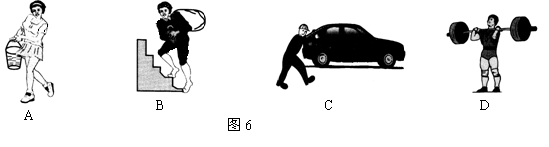
\includegraphics[scale=1]{figures/图片1.png} 
\begin{choices}
\choice 提着水桶在水平地面上匀速前进
\choice 扛着米袋慢慢爬上楼梯 
\choice 用力推汽车,汽车没动
\choice 举着杠铃原地不动
\end{choices}

\question



\end{questions}












\begin{advanceexercises}
\section{提高题}



\end{advanceexercises}

\ThisCenterWallPaper{1}{教案模板-3.pdf}

\end{document}



